\section{Theoretical and Simulation Analysis}
\label{sec:analysis}

We will be dealing with the simulation and theoretical analysis at the same time. Next we present a table of constans that will be used.

\begin{table}[h]
    \centering
    \begin{tabular}{|l|c|c|}
    \hline
    {\bf Name} & {\bf Value} & {\bf Units} \\ \hline
    $R_1$ & $33.7$ & $k\Omega$ [kOhms] \\ \hline
    $R_2$ & $3.6$ & $k\Omega$ [kOhms] \\ \hline
    $R_C$ & $3.8$ & $k\Omega$ [kOhms] \\ \hline
    $R_E$ & $200$ & $\Omega$ [Ohms] \\ \hline
    $R_{out}$ & $400$ & $\Omega$ [Ohms] \\ \hline
    $C_{in}$ & $800$ & $\mu F$ [$\mu$Farads]\\ \hline
    $C_E$ & $800$ & $\mu F$ [$\mu$Farads] \\ \hline
    $C_o$ & $600$ & $\mu F$ [$\mu$Farads] \\ \hline
    \end{tabular}
    \caption{Constants Values}
    \label{tab:constants}
\end{table}

\subsection{Gain Stage}
\label{subsec:stat}

The Gain Stage of the circuit is responsible for insuring a high input voltage so the input signal is not degradated through the circuit. It has ana elevated gain and is the part responsible for signal amplification.

There are 3 types of elements: a NPN BJT, resistors and capacitors.

The first capacitor, $C_{in}$, is a coupling capacitor, as it acts as a DC Block, so that $V_{in}$ doesn't impose a DC component of 0, that would change the OP of the transistor.

The second capacitor, $C_E$, acts as a bypass capacitor, for it ensures that for low frequencies all the current flows through $R_E$, and for high frequencies, it passes through the capacitor.

The output impedance of this stage ($Z_{O1}$) is high.

\subsection{Output Stage}

The Gain Stage has a high $Z_{O1}$ soto counter this, we connect a circuit with low output impedance to the first one. This circuit presents similar components but with very distinct results.

Instead of a NPN BJT, we use a PNP BJT, because it has a higher $\beta_F$, which lowers the output impedance. 

Another capacitor, $C_o$, is used with a similar goal as the previous coupling capacitor. If we didn't use such component, the gain stage would impose a DC voltage of 0 to the second stage, which would ruin the transistor's OP. 

As we'll see, we end up with a lower output impedance in this stage and a higher input impedance (when compared to the output impedance of the gain stage).

When combining both stages, we need to ensure that there is a compatibility  between the impedances, the input impedance of the second stage should be much greater than the output impedance of the first one. 


\clearpage
\subsection{Theoretical Analysis}
\label{subsec:Req}

In the theoretical analysis we will evaluate the four impedances associated with the two stages ($Z_{I1}, Z_{O1}, Z_{I2}$ and $Z_{O2}$) and the two gains in each stage ($A_{V1}$ and $A_{V2}$).

\subsubsection{Impedances}

In the fist stage we can finde the input and output impedances (\{$Z_{I1}$, $Z_{O1}$\})using KVL and KCL.

\begin{equation}
    Z_{I1}=R_B // r_{\pi 1}
\end{equation}
where $R_B=R_1 // R_2$.


We assume $R_E \simeq 0$ (capacitors are short-circuted). 
The first stage input matches the total input impedance of the circuit.

The first stage output impedance can be obtained by:

\begin{equation}
    Z_{O1}=r_o // R_C  
\end{equation}

For the second stage, by analysing the circuit we get:

\begin{equation}
    Z_{I2}=\frac{(g_{m2}+g_{\pi2}+g_{o2}+g_{E2})}{g_{\pi2}(g_{\pi2}+g_{o2}+g_{E2})}
\end{equation}

\begin{equation}
    Z_{O2}=\frac{1}{(g_{m2}+g_{\pi2}+g_{o2}+g_{E2})}
\end{equation}

And finally, the total output impedance:

\begin{equation}
    Z_{OT}=\frac{v_o}{i_o}=\frac{1}{g_{o2}+g_{m2}\frac{r_{\pi2}}{r_{\pi2}+Z_{O1}}+g_{E2}+\frac{1}{r_{\pi2}+Z_{O1}}}
\end{equation}

The 4 values are presented below,

\begin{table}[h]
    \centering
    \begin{tabular}{|l|c|}
    \hline
    {\bf Impedances} & {\bf Ohms ($\Omega$)} \\ \hline
    $Z_{I1}$	&	1290.209759\\\hline
$Z_{O1}$	&	3411.452239\\\hline
$Z_{I2}$	&	37245.135442\\\hline
$Z_{O2}$	&	1.375831\\\hline
$Z_{OT}$	&	15.566019\\\hline

    \end{tabular}
    \caption{Theoretical Impedances}
    \label{tab:theo_imp}
\end{table}

Remembering that $Z_{O1}$ needs to be  much lower than $Z_{I2}$, we end up with good results. This is needed so that there is no signal degradation or loss between these stages.


\subsubsection{Gain}

To calculate the total gain ($A_{V}$) we performed a simple multiplication $A_V=A_{V1}A_{V2}$. The real interaction between both stages is negligible, and so we can compute the gain as if it was the total gain of both separate stages.

\begin{table}[h]
\parbox{.4\linewidth}{
  \centering
    \begin{tabular}{|l|c|}
    \hline
    {\bf Gain} & {\bf Value} \\ \hline
    $G_1$	&	-264.565721\\\hline
$G_2$	&	0.991532\\\hline
$G_T$	&	-252.275561\\\hline
$G_{T_{dB}}$	&	48.037504\\\hline

    \end{tabular}
    \caption{Theoretical upper gain bound results}
    \label{tab:theo_gains_high}
  }
  \hfill
  \parbox{.4\textwidth}{
  \centering  
  \begin{tabular}{|c|c|}
    \hline    
    {\bf Gain} & {\bf Value} \\ \hline
    $G_1$	&	-17.126226\\\hline
$G_2$	&	0.991532\\\hline
$G_T$	&	-16.330643\\\hline
$G_{T_{dB}}$	&	24.260066\\\hline

  \end{tabular}
  \caption{Theoretical lower gain bound results}
  \label{tab:theo_gains_low}
  }
  \end{table}
  


To acquire a better comparison between theory and simulation, besides this aproach, that considers the gain to be constant through all the frequencies , we also performed the \textit{Time constant method} for the lower cut-off frequency.

We calculate the lower cut-off frequency ($\omega_L=2\pi f_{CO_L}$) as,

\begin{equation}
    \omega_L=1/{R_{eq_i}C_i} + 1/{R_{eq_e}C_e} + 1/{R_{eq_o}C_o}
    \implies f_{CO_L}=2\pi w_L
\end{equation}

where $R_{eq}\equiv$ equivalent resistor as seen by each capacitor when the others are short-circuits.

We have,

\begin{equation}
    R_{eq_{in}} = R_{in}+Z_{I1}
\end{equation}

\begin{equation}
    R_{eq_e} = R_E // (\frac{1}{\frac{1}{R_s||R_B+r_{\pi}}+\frac{g_m r_{\pi}}{R_s||R_B+r_{\pi}}}) \simeq R_E//(\frac{r_{\pi}+R_s||R_B}{r_{\pi}}\frac{1}{g_m}) \simeq 1/g_{m}
\end{equation}

\begin{equation}
    R_{eq_o}=R_L+Z_{O}
\end{equation}

The theoretical value of the lower cut-off frequency is presented in the table below.

\begin{table}[h]
    \centering
    \begin{tabular}{|l|c|}
    \hline
    {\bf Name} & {\bf Value [Hz]} \\ \hline
    Lower CO freq	&	28.296662\\\hline

    \end{tabular}
    \caption{Theoretical Lower Cut-off frequency}
    \label{tab:theo_CO_freq}
\end{table}

\pagebreak

\subsection{Simulation Analysis}
\label{subsec:Req}

In the Simulation Analysis, we want to get the two impedances associated with the circuit, the two cut-off frequencies, $f_{CO_L}$ and $f_{CO_H}$, the bandwidth and the total gain, $A_V$.
We also check whether the BJT's are on the Forward Active Region (FAR), by comparing $V_{CE}$ and $V_{BE}$ for the NPN, and, analogously, $V_{EC}$ and $V_{EB}$ for PNP. 


\begin{table}[h]
    \centering
    \begin{tabular}{|c|c|}
    \hline
    {\bf Name} & {\bf Value} \\ \hline
    \input{NPN_tab.tex}
    \end{tabular}
    \caption{NPN voltages and FAR confirmation}
    \label{tab:NPN}
\end{table}

\begin{table}[h]
    \centering
    \begin{tabular}{|c|c|}
    \hline
    {\bf Name} & {\bf Value} \\ \hline
    \input{PNP_tab.tex}
    \end{tabular}
    \caption{PNP voltages and FAR confirmation}
    \label{tab:PNP}
\end{table}


The results are presented in the table below:

\begin{table}[h]
    \centering
    \begin{tabular}{|c|c|c|}
    \hline
    {\bf Name} & {\bf Value} & {\bf Units}\\ \hline
    \input{gain_band_COfreq_tab.tex}
    \end{tabular}
    \caption{Simulation results}
    \label{tab:sim_results}
\end{table}


\subsubsection{Coupling Capacitors}

To be able to analyse the circuit, we need to understand the Coupling Capacitor's behaviour. In our amplifier we have two coupling capacitors, $C_O$ and $C_{in}$, but due to the analog nature of the functions, we will focus on the capacitor $C_{in}$.
The two figures of the frequency response analysis are presented below.

\begin{figure}[h]
\centering
\begin{subfigure}{.5\textwidth}
    \centering
    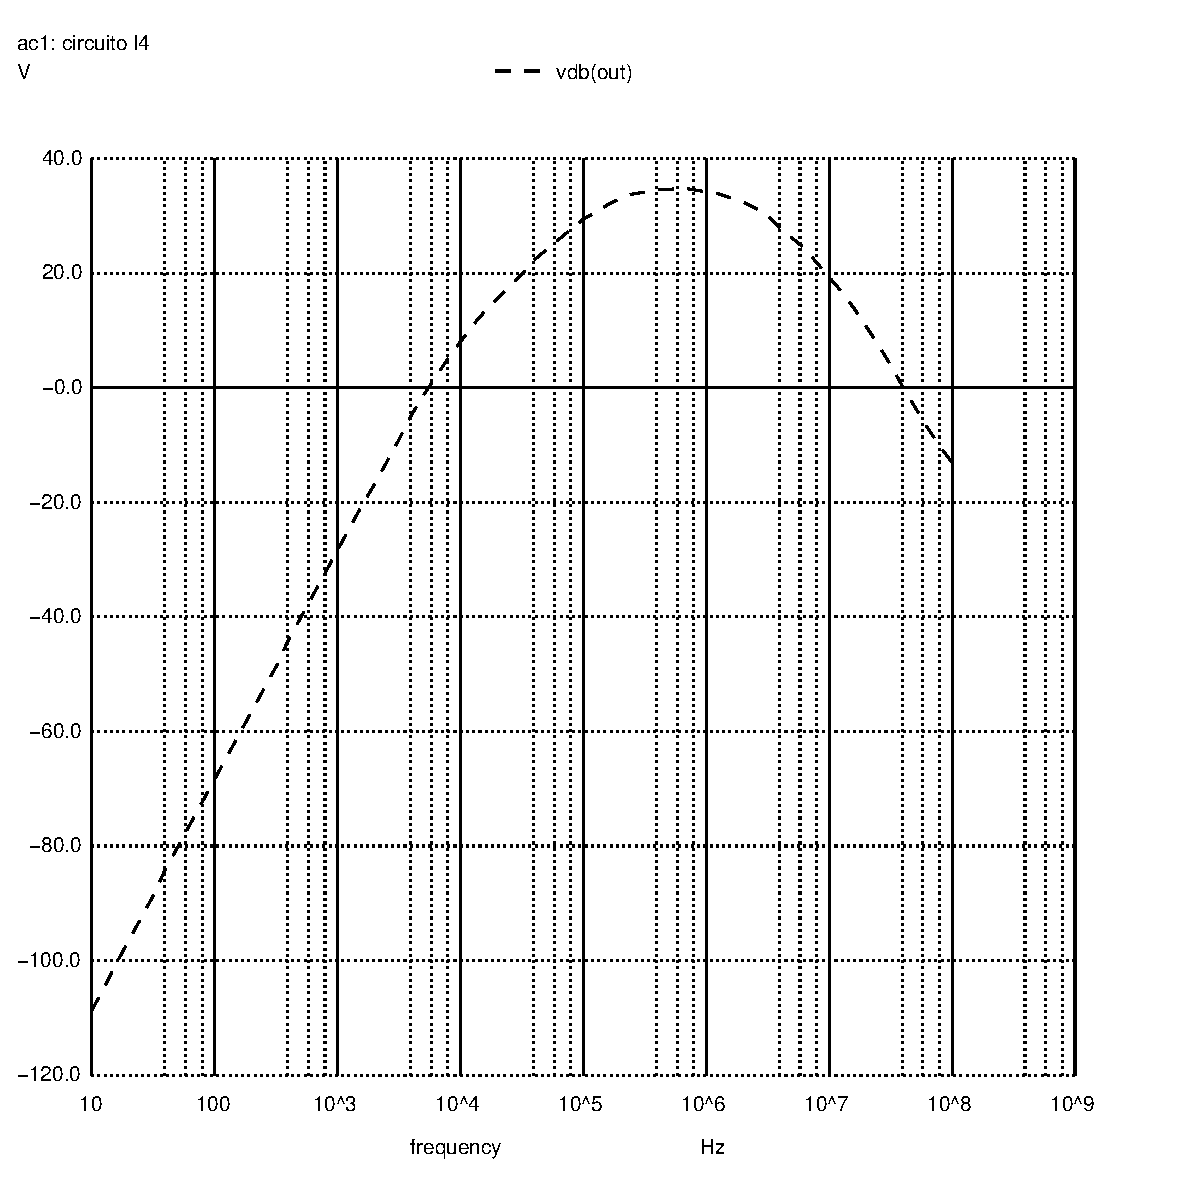
\includegraphics[scale=0.33]{images/cilow_1n.eps}
    \caption{$C_i$ low (1$nF$)}
\end{subfigure}%
\begin{subfigure}{.5\textwidth}
    \centering
    \includegraphics[scale=0.33]{images/cihigh_1.eps}
    \caption{$C_i$ high (1$F$)}
\end{subfigure}
\caption{$C_{in}$ influence}
\end{figure}

\pagebreak

We can see that the increase of the capacitance pushes the cut-off frequency to the left and, without altering the higher cut-off frequency, anticipating it, wich generates a larger bandwidth.
As discussed previously, as $\omega \to 0$, $Z(C_{in}) \to \inf$, this is not surprising, so this capacitor prevents the transistor from entering the cut-off regions or the saturation, by blocking the DC component of the Audio In source. This helps the transistor operate at lower frequencies by mantaining the OP of the transistor, as $C_{in}$ increases.

\subsubsection{Bypass Capacitor}

The two figures of the frequency response analysis, by changing the parameter $C_E$, are presented below.

\begin{figure}[h]
\centering
\begin{subfigure}{.5\textwidth}
    \centering
    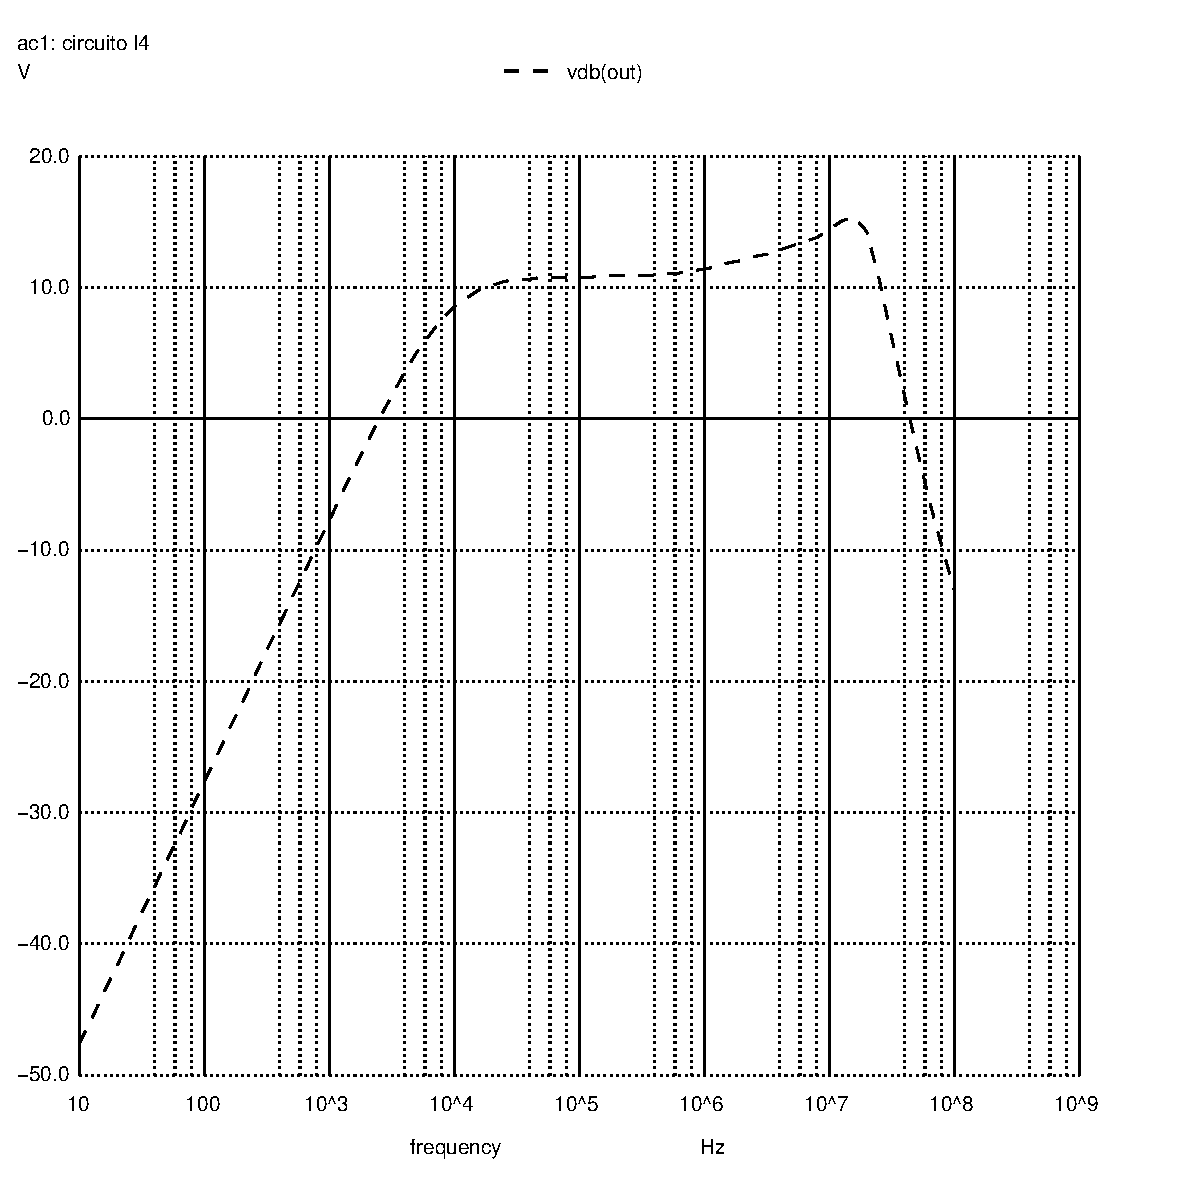
\includegraphics[scale=0.33]{images/celow_1n.eps}
    \caption{Low $C_E$ effect on Gain (1$nF$)}
\end{subfigure}%
\begin{subfigure}{.5\textwidth}
    \centering
    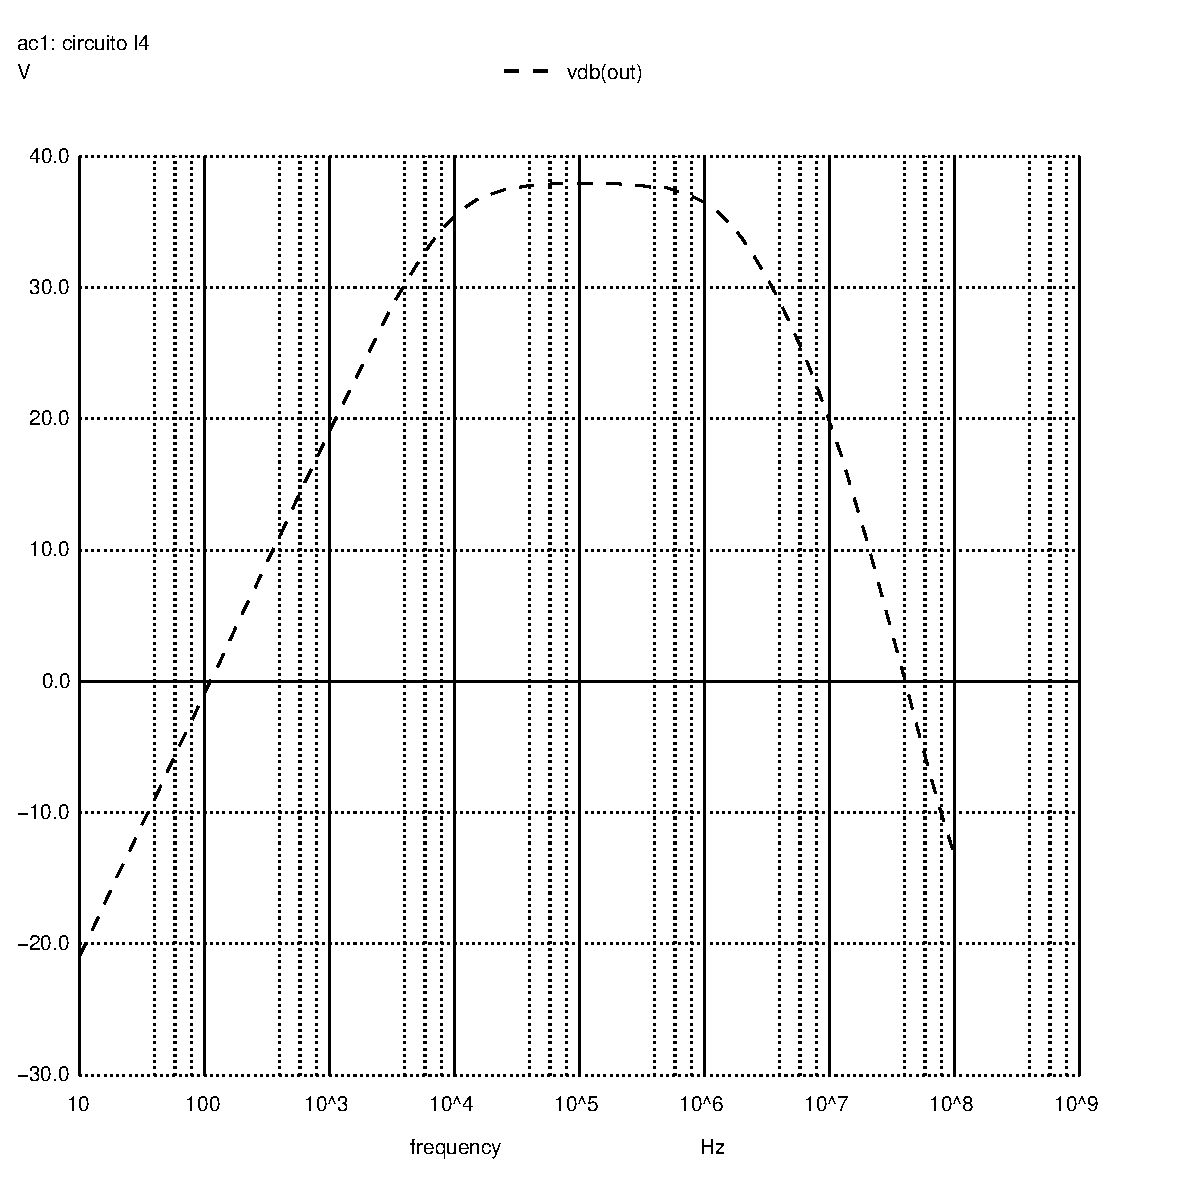
\includegraphics[scale=0.33]{images/cehigh_1.eps}
    \caption{High $C_E$ effect on Gain (1$F$)}
\end{subfigure}
\caption{$C_E$ influence}
\end{figure}

Due to the placement of the bypass capacitor in parallel with $R_E$, this resistor becomes short for high and medium freuqencies. The amplifier's first stage gain being inversely dependent on this resistance leads to the bypass capacitor playing an extremelly importante role in maximizing the gain for high and medium frequencies.

\subsubsection{$R_C$}

To conclude, we need to analyse the role of $R_C$ on the total gain of the circuit.
We also present assymptotical situations in order to fully understand that behaviour.

\begin{figure}[h]
\centering
\begin{subfigure}{.5\textwidth}
    \centering
    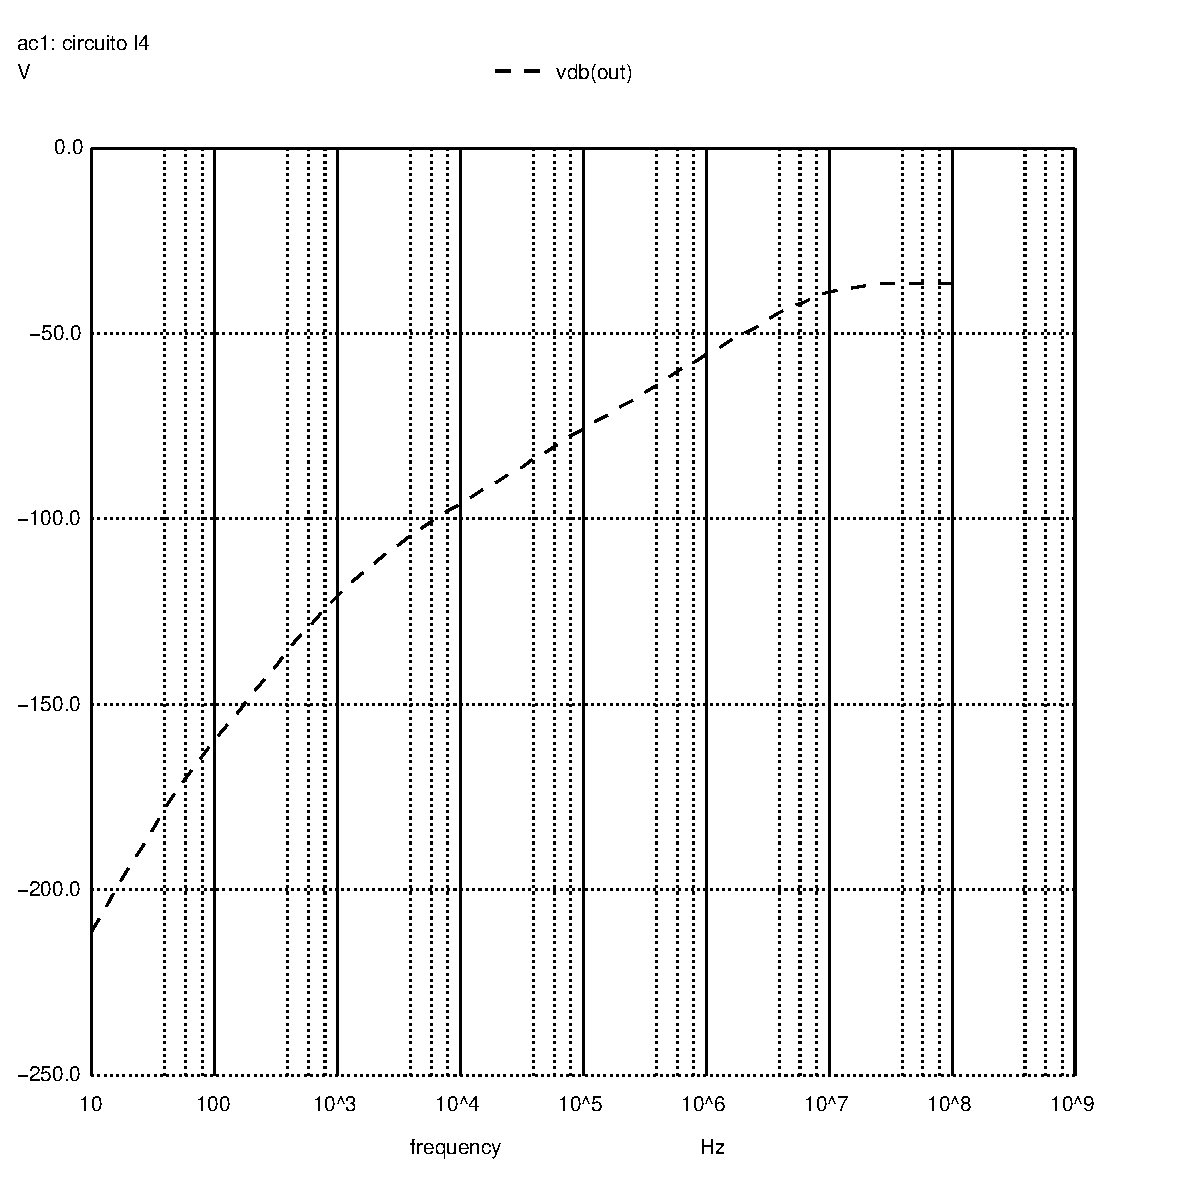
\includegraphics[scale=0.33]{images/rclow_10.eps}
    \caption{Low $R_C$ effect (on the Gain) (10$\Omega$)}
\end{subfigure}%
\begin{subfigure}{.5\textwidth}
    \centering
    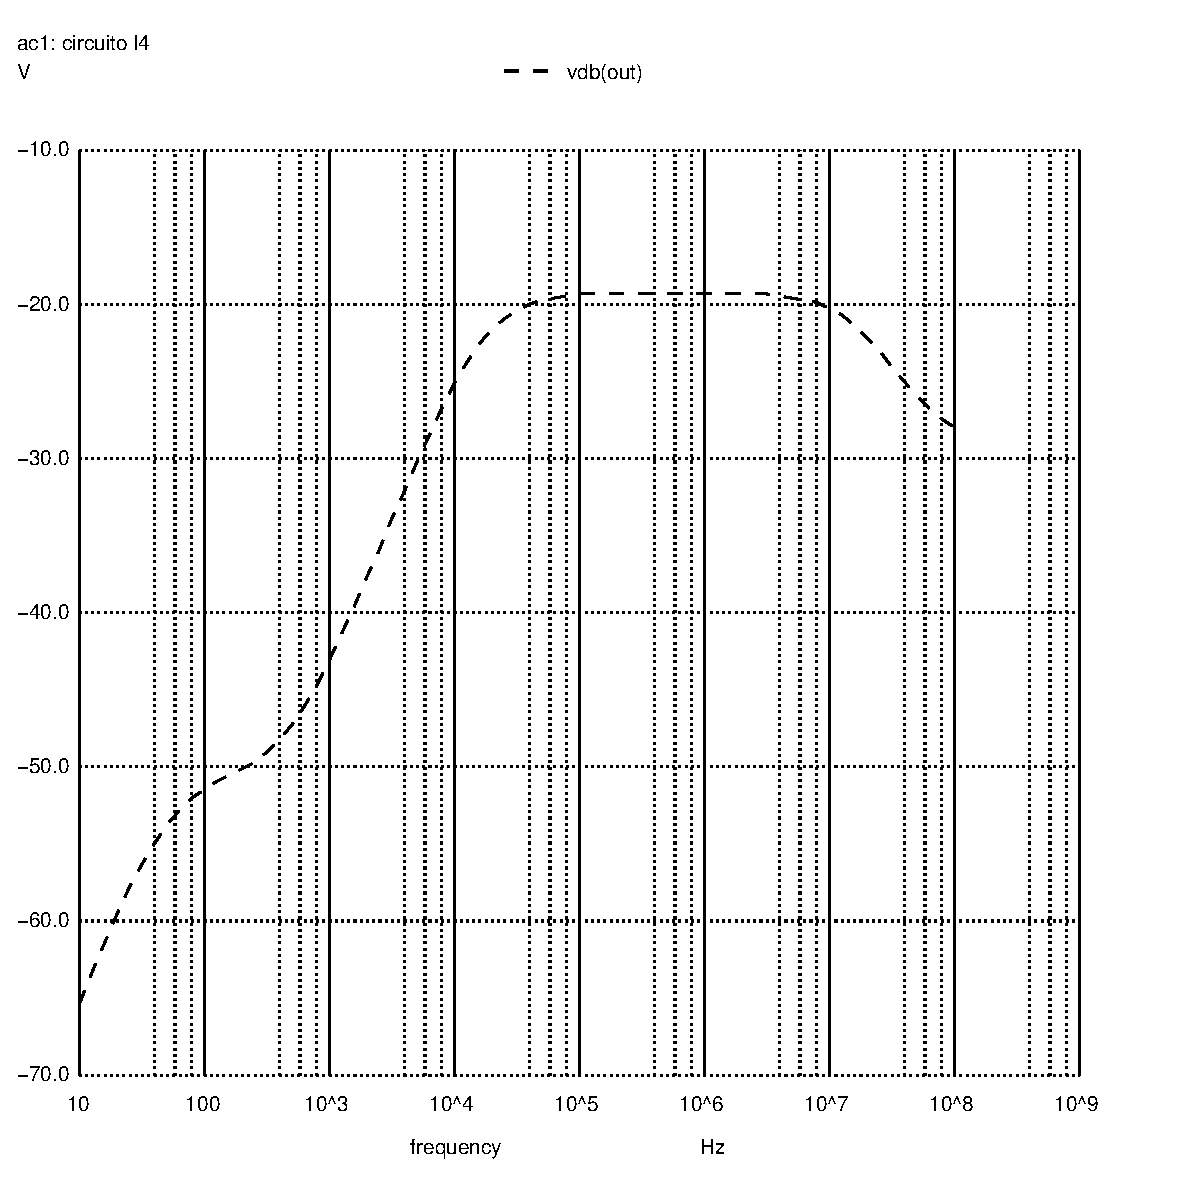
\includegraphics[scale=0.33]{images/rchigh_100k.eps}
    \caption{High $R_C$ effect on Gain (10$k\Omega$)}
    \label{fig:RC_High}
\end{subfigure}
\caption{$R_C$ influence (on the Gain)}
\end{figure}

We can see that the gain increases with $R_C$ and also antecipates de passband. This behaviour matches the predictions given by the theoretical analysis on the gain, due to being proporcional to $R_C$.

To guarantee a high compatibility with speakers and AUDIO IN, we simulate the input and output impedances of the circuit. The goog compatibility is guaranteed with a high input impedance, $Z_I$, and a low output impedance, $Z_O$. The results are presented in the tables below.

\begin{table}[h]
    \centering
    \begin{tabular}{|l|c|}
    \hline
    {\bf Name} & {\bf Value [$\Omega$]} \\ \hline
    Input Imp & 999.991 + -723.534 j\\ \hline

    \end{tabular}
    \caption{Simulation Input Impedance}
    \label{tab:simulation_input_imp}
\end{table}

\begin{table}[h]
    \centering
    \begin{tabular}{|l|c|}
    \hline
    {\bf Name} & {\bf Value [$\Omega$]} \\ \hline
    Output Imp & 680.05 + -466.901 j\\ \hline

    \end{tabular}
    \caption{Simulation Output Impedance}
    \label{tab:simulation_output_imp}
\end{table}

In similarity with the theoretical analysis, the simulation gives off a slightly high output impedance. This is due to the compromises needed fot the merit system.
\pagebreak

\subsection{Comparison}
\label{subsec:comparison}

We are now going to compare theoretical and simulation values.

\vspace{-2.5cm}

\begin{figure}[h]
\centering
\begin{subfigure}{.5\textwidth}
    \centering
    \vspace{2.8 cm}
    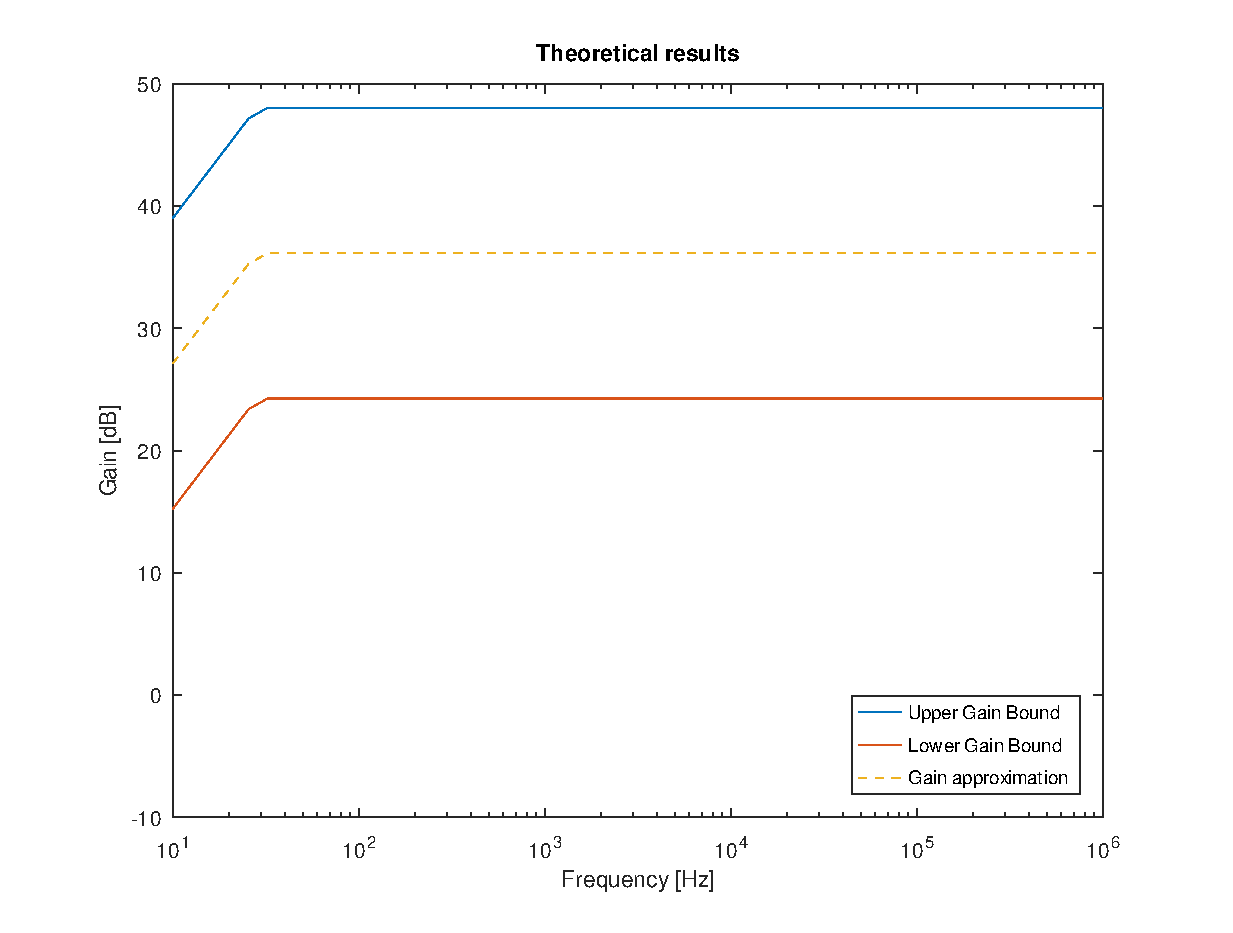
\includegraphics[scale=0.4]{theo_results.eps}
    \caption{Theoretical Gain}
\end{subfigure}%
\begin{subfigure}{.5\textwidth}
    \centering
    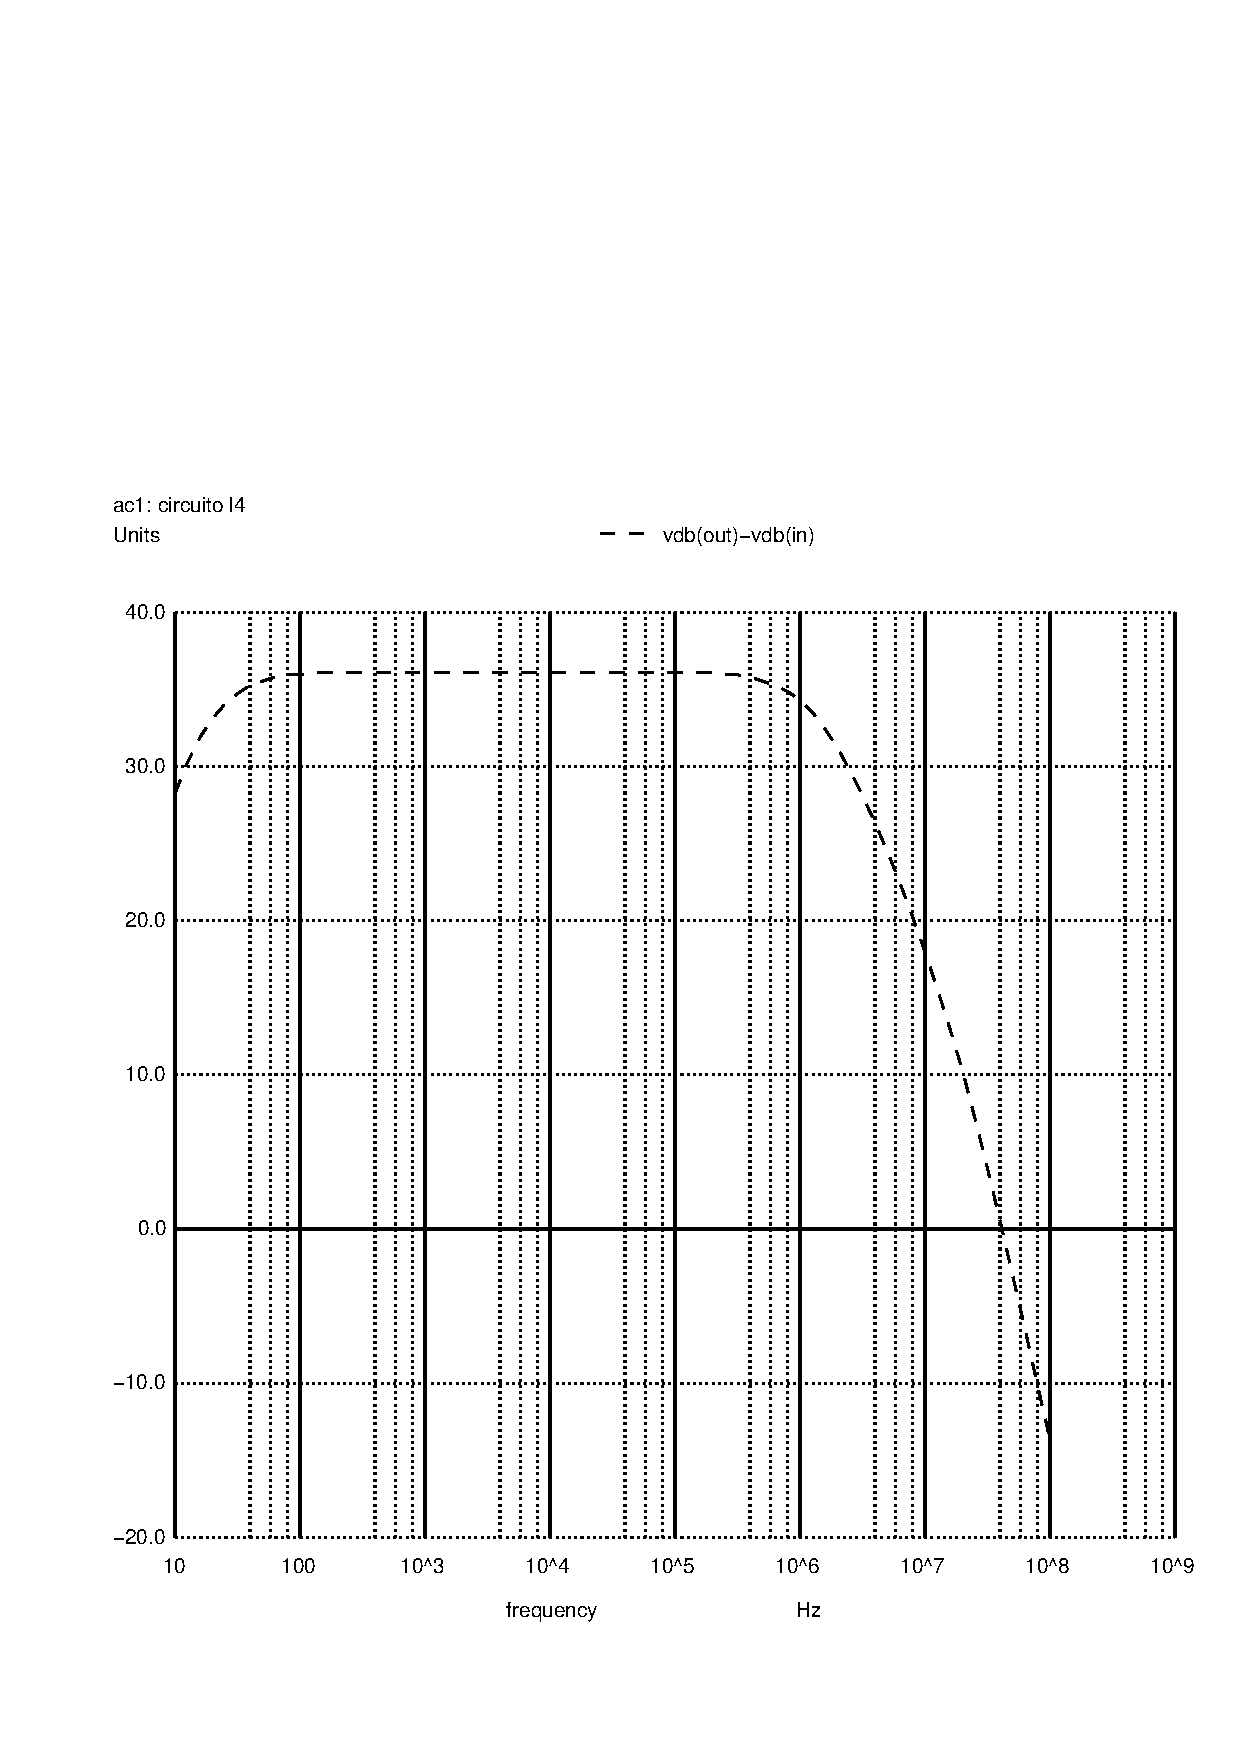
\includegraphics[scale=0.33]{vo2f.pdf}
    \caption{Simulation Gain}
\end{subfigure}
\caption{Gain}
\label{fig:Gain}
\end{figure}

Above we can see theoretical and simulation graphs of the gain.

In this case, the comparison of the shape can only be done on the left side, since we don't have the theoretical higher cut-off frequency. For this reason, there's no point in plotting the theoretical gain any further than $1 MHz$.

The theoretical analysis takes in acount that all capacitors are short-circuted or open-circuted, leading to two different plots one in blue and the other one in orange, respectively. This leaves us with a region of acceptance for the simulation gain, that fits in this region for the interval in study. The yellow plot is the average gain, wich should be a better approximation of the real gain. Considering both graphs we can also comment on their similar shape that confirmes the match of our theoretical aproach. Looking back on the studied values of each the theoretical and the simulation analysis ($Z_I$ and $Z_O$, $A_v$ and $f_{CO_L}$), we can confirm that they have the similar orders of magnitude, wich gives us an aproximation within reason.

\section{Merit Results}
\label{sec:merit}

Using the results obtained through the Ngspice simulation (see Section \ref{subsec:comparison}) and having in mind that we used the data shown in Section \ref{sec:introduction}, we can compute the price and the merit using the \textit{formulae} given in the lab assignment:

The price obtained was 2242.01 and the merit was 1965.72.

We chose to firstly understand what would be produced by each component when its values changed dramatically. So we analysed the circuit \textit{assymptotically} in order to acquire a bigger notion of what would be influenced by each component.

After having a good notion about that, we just made small adjustments get our results as perfect as possible, which made the merit rise. By using this approach, the cost was left as a second thought.

To end, we started decreasing the cost until we found what we thought was a good balance, giving the results presented above.


